\documentclass[10pt]{article}
\usepackage[margin=0.7in]{geometry}
\usepackage{amsmath, amssymb}
\usepackage{graphicx}
\usepackage{booktabs}
\usepackage{hyperref}
\usepackage{float}
\usepackage{multicol}
\setlength{\parindent}{0pt}
\setlength{\parskip}{3pt}

\hypersetup{colorlinks=true, linkcolor=blue, urlcolor=blue, citecolor=blue}

\title{Comparing Scientific ML Methods for Nonlinear ODE Dynamics}
\author{Xuanyou Liu (NetID: XLM6838)}
\date{ELE\_ENG 395 Scientific Machine Learning, Final Project, \today}

\begin{document}
\maketitle

\textbf{Abstract.}
This project benchmarks data-driven and physics-structured models for learning nonlinear ODE dynamics from noisy trajectories.
I evaluate baseline MLPs, Neural ODE rollouts, and a structured Lagrangian neural network (LNN) on two course systems: Van der Pol and the simple pendulum.
Key findings: (1) the LNN reduces trajectory RMSE by two orders of magnitude over black-box baselines while nearly conserving energy; (2) on single-trajectory Van der Pol fitting, a compact MLP outperforms long-horizon rollout training; (3) deeper networks are not uniformly better due to spectral bias and optimization difficulty.

\section*{1. Introduction}
Learning dynamics from noisy observations is a central problem in scientific machine learning.
Black-box regressors fit data efficiently but may violate dynamical consistency; rollout-based models are physically motivated but accumulate integration error; physics-structured models exploit known invariances at the cost of specialization.
This project extends Chapters~5 and~7 homework into a unified benchmark with reproducible code, common metrics, and direct comparison across model families.

\textbf{Objective.}
Compare baseline MLPs, Neural ODEs, and a structured LNN in terms of trajectory RMSE, energy conservation, and training cost.

\section*{2. Method}

\textbf{Van der Pol} ($\dot{z}{=}v,\;\dot{v}{=}\mu(1{-}z^2)v{-}z,\;\mu{=}1$):
RK4 on $t\!\in\![0,20]$, $\Delta t{=}0.1$, Gaussian noise $\sigma{=}0.1$.
MLP capacity study (2$\times$32, 6$\times$32, 2$\times$128) and Neural ODE rollout.

\textbf{Pendulum} ($\ddot{\theta}{+}\frac{g}{\ell}\sin\theta{=}0,\;\frac{g}{\ell}{=}9.81$):
80 RK4 trajectories on $t\!\in\![0,10]$ (400 steps), noise $\sigma{=}0.02$, split 56/12/12.
One-step baseline MLP with autoregressive rollout, Neural ODE, and structured LNN trained on finite-difference acceleration targets via $\ddot{\theta}_{\text{pred}}{=}{-}\frac{dV_W}{d\theta}$.

\section*{3. Results}

\begin{table}[H]
\centering
\small
\caption{Trajectory RMSE, parameter count, and training time.}
\begin{tabular}{@{}llccrc@{}}
\toprule
System & Model & St.~1 RMSE & St.~2 RMSE & Params & Time (s) \\
\midrule
Van der Pol & Baseline MLP & 0.053 ($z$) & 0.239 ($v$) & 1\,153 & 0.4 \\
Van der Pol & Neural ODE & 0.188 ($z$) & 0.383 ($v$) & 4\,482 & 23.7 \\
\midrule
Pendulum & Baseline MLP & 0.496 ($\theta$) & 1.511 ($\omega$) & 4\,482 & 2.7 \\
Pendulum & Neural ODE & 0.188 ($\theta$) & 0.499 ($\omega$) & 4\,482 & 52.8 \\
Pendulum & Structured LNN & \textbf{0.006} ($\theta$) & \textbf{0.017} ($\omega$) & 8\,513 & 12.1 \\
\bottomrule
\end{tabular}
\end{table}

\textbf{Capacity and spectral bias.}
On Van der Pol, the compact 2$\times$32 MLP (1\,153 params) outperformed both the deep 6$\times$32 (RMSE 0.895) and wide 2$\times$128 (RMSE 0.104) variants.
The deep model failed to fit oscillatory structure, consistent with spectral bias and vanishing-gradient effects in deeper tanh networks.

\textbf{Energy conservation.}
For pendulum, the LNN rollout shows energy drift std of 0.002 versus 0.553 for Neural ODE, demonstrating that the physics-structured architecture implicitly preserves the system's Hamiltonian structure.

\begin{figure}[H]
\centering
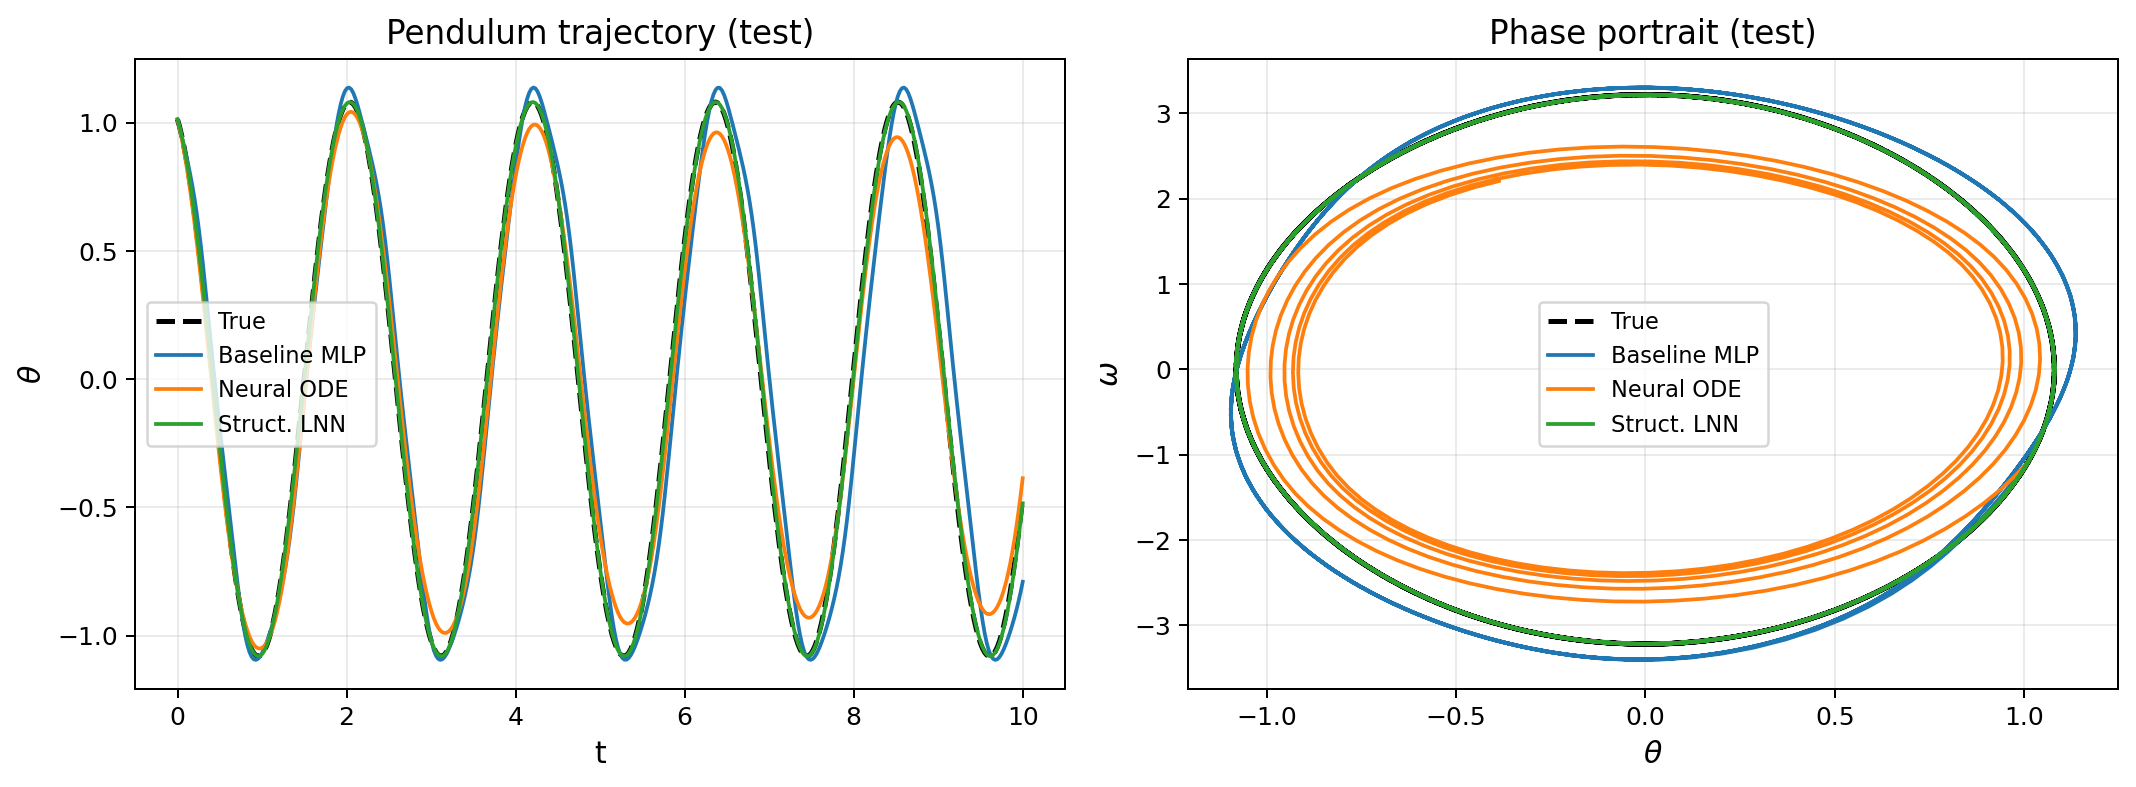
\includegraphics[width=0.98\linewidth]{../code/figures/pendulum_model_comparison.png}
\caption{Representative pendulum test trajectory (left) and phase portrait (right). The structured LNN closely tracks the true dynamics while baseline and Neural ODE drift.}
\end{figure}

\begin{figure}[H]
\centering
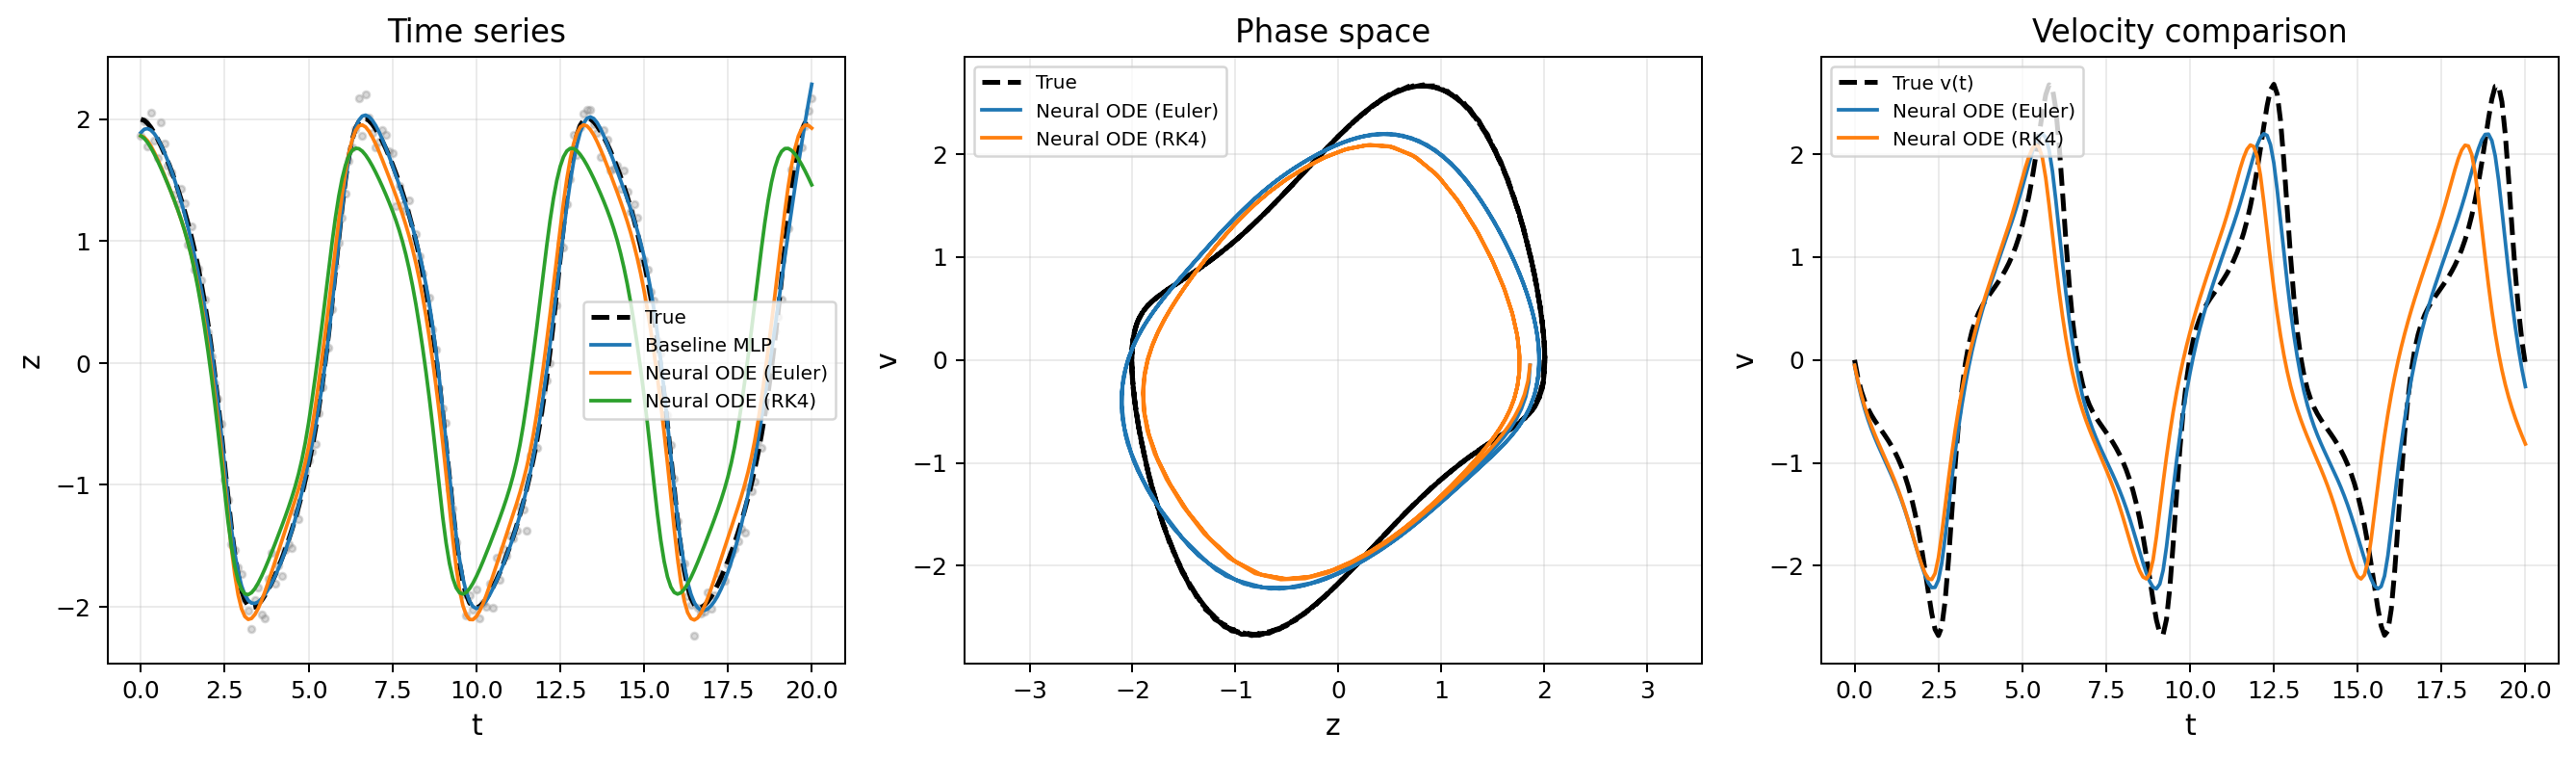
\includegraphics[width=0.98\linewidth]{../code/figures/vdp_model_comparison.png}
\caption{Van der Pol: time series, phase space, and velocity comparisons between baseline MLP, Neural ODE (Euler), and Neural ODE (RK4 evaluation).}
\end{figure}

\section*{4. Discussion}

Three findings stand out.
First, model capacity does not automatically improve fitting: the compact MLP outperformed larger variants on Van der Pol, highlighting that architecture search matters.
Second, integration error compounds: the Neural ODE trained with Euler rollout underperformed direct regression on a single trajectory, though it better captured phase-space structure.
Third, when correct physics structure is available, the inductive bias is decisive: the pendulum LNN reduced RMSE by nearly 100$\times$ and preserved energy conservation.

\textbf{Limitations.}
Van der Pol uses one initial condition and first-order Euler for Neural ODE training; both choices disadvantage rollout models.
The LNN assumes known kinetic energy form, which may not generalize to systems without such decomposition.

\textbf{Future work.}
Higher-order differentiable integrators for Neural ODE training, PINN-style residual constraints, and extension to chaotic systems (Lorenz, double pendulum).

\textbf{Reproducibility.}
All code: \url{https://github.com/Xuanyou-Liu/ELE_ENG-395-Final-Project}. Run \texttt{bash scripts/reproduce\_all.sh}.

\end{document}
